\subsection{Research Questions and Method Overview}

The methodology studies the ability of RAGPoisoon to act as a red-teaming benchmark for LLM-powered reccomender systems. The main question it raises is local reccomendation system that combines retrieval, ranking, LLM reranking and full experiement artifact with its traces can get show real mesurable effects when the data is poisonned. We thus raise three research questions: can the objectively compare the clean and poisoned reccomendation while kepping the same user data and evaluation logic fixed, can it use the same code to represent all attack families succesfully and finally, can the resulting behavior be computed correctly enough to trust the shared metrics from every run and label whether they are successfuly poisoned based on the reccomendation quality \cite{ragpoisonlab_repo,li2016factorizationpoison,fang2020influencepoison,nguyen2024manipulatingrecsys}.

The comparing method, as briefly discussed previously, is simply based on baseline/attacked design where a movielens user profile and a movie set is fixed. We simply request reccomendation from both indices and comput the metrics of both resulting lists then store their deltas. The method, from an engineering platform, helps study the reproducibility of the run so that a solution can be found to fix it and avoid unproven broad claims. It is also alligned with the exact situation a retrievall augmented system can be found in, where the attacker changes the retrieved content and the reccomender uses that data as if it was partof the original documents \cite{ragpoisonlab_repo,zhong2023retrievalcorpora,zou2025poisonedrag_usenix}.

The benchmark methodology observes from 3 specific points. The first one is at user level where we compare results of both pipelines on one user, the second is a fulll dataset run with one attack type, one specific retrieval and ranking mode and one attacker and its victim. The last one, and the most relevant, is as we will call it a full matrix run that will run all attack types with all elected models. These points of observation are not specifically separated but are actual the same, the fiirst 2 points being a sample of a full matrix run. a single single user level run can display the power of our tool while a full matrix gives us all the data we need to complete this thesis \cite{ragpoisonlab_repo}.

The variability of attack methods, models and policies doesn't try to pprove the strenght of a model or an attack compared to another one but rather asks whether the current implemented framework can viably show the strength and weaknesses of each of them successfully making it perfect for the ppurpose of this thesis. The choice of the datset stays purely for its small size. It helps us shorten the legnth of each run and keep it at a viable 8 hours per run \cite{ragpoisonlab_repo}.

\subsection{Threat Model}

The threat model always assumes a close environement where the attacker can only influence indexed movies before the retrieval index is created. The influence of the attacks can be seen in the local corpus transformations but not in the user ratings history since that would defeat the purpose of poisonning the recommendation. It does not affect the code made for evaluation and never affects the recommender service or changes model behavior. The victim system, which owns the reccomendation pipeline, will build the user queries, retrieves the candidates from the index, ranks and reranks them then retruns the top-$k$ list \cite{ragpoisonlab_repo,zhong2023retrievalcorpora,zou2025poisonedrag_usenix,zhang2024humanimperceptible}. 

Based on the different attack families the attacker will have a different objective. For targeted promotion, the objective is that a chosen movie, which would never be reccomended to a user, appears in the top-$k$ reccomender list more often. For prompt injection, we try to study how injected metadata and prompt modification can affect the retrieval and reranking path. Untargeted degradation the other hand doesnt have a specific item to promote, but rather has as an objective to lower the reccomendation quality. Due to the different objectives of each attack it iis hard to mesure them and summerize them under one same score \cite{ragpoisonlab_repo,li2016factorizationpoison,nguyen2024manipulatingrecsys,wang2024recpoisonsurvey}.

Though being a simulation of real world attacks, RAGPoison specifically excludes actions like test phishing, credential theft, external service compromise or other attacks as they are external to our scope. the attack implementation stays inside the MovieLens dataset corpus, and Section~\ref{sec:system-design} identifies that clearly. We thus want to clarify that working under the current conditions the MovieLens setting doesn't capture all the effect of multimodal or commerce recommenders. The boundary we set doesn't allow us to try for those settings as the priority set was security \cite{ragpoisonlab_repo,perez2022redteaming,mazeika2024harmbench}.

The attacker can only affect existing data. It cannot create new users or add in items, it is bound the the MovieLens derived item records like the title, genres and synopsis fields used by retrieval. This is relevant because it ensures that all results are truly derieved from our dataset, and that the poisonned corpus is relevant to the expected result alowwing use to correctly comppute the metrics \cite{ragpoisonlab_repo,harper2015movielens}

The victim syystem has the ability to use either deterministic or LLM Reranking, though deterministic is only used as a fallback we still include the testing of it in some of our attacks where it is more relevant. This is important because LLM-powered recommenders can fail because posioned text changes the the first retrieval step or because it affected the LLM that reads the description of the candidates during reranking. the predetermined items are sent to the LLM to re-order, and never has to generate its oown reccomendation from scratch keeping the cost price effective and messurable \cite{ragpoisonlab_repo,hou2024llmrankers,sun2024rankgpt}

\subsection{Attack Families}

To better display all attack families Figure~\ref{fig:attack-pipeline} shows how all three are implemented \cite{ragpoisonlab_repo}.

Targeted promotion allows the attacker to choose or auto select a targeted movie and modify the indexed documents to give the selected item a higher chance to appear in the top recommendations making it the most direct attack family. all implemented poison metadata is recorded alongside the keyword boosting policy value. It is supposed to answer the following question: Does the targeted movie enter the top-$k$ under the selected conditions? It uses a supporting metric, ASR@K,  to answer that question on top of the previously cited metrics, as the attack can be successful even if HR or NDCG doesn't seem to change much be cause the objective is to push one movie or item to the top \cite{ragpoisonlab_repo,nguyen2024manipulatingrecsys,wang2024recpoisonsurvey}.

Prompt injection studies a similar risk with some slight differences. When using RAG, the retrieved text is consummed later on by the LLM so it leaves an opening for malicious instuction like text to be injected in one of the retrieved items \cite{greshake2023indirectpi,yi2025bipia}. Prompt injection are thus represented as controlled benchmark records where we inject and store a payload, wheteher through the LLM or deterministically and then store it in \texttt{poison\_payload}. In Section~\ref{sec:system-design} we show the exact benchmark payloads used. For this family the question is whether the injected item can reach the retrieval/ranking path and help push a certain item to the top-$k$ reccomendations. The ASR matric is thus useful and necessary for this attack too \cite{ragpoisonlab_repo,greshake2023indirectpi,yi2025bipia,nguyen2024manipulatingrecsys,wang2024recpoisonsurvey}.

untargeted on the other hand is, as said previously, more for quality damage as it doesn't promote any specific items but rather hurt select documents so that general results becomes useless for reccomendation. The current code implements this attack by adding or rather making harmful transformation by modifying the genres or replacing the synospis with non relevant text \cite{ragpoisonlab_repo}. The question it raises is how much is top-$k$ list affected in keeping the relevant reccomended items and how llow are they pushed down the list. contrary to the previous attacks here ASR is not relevant so HR NDCG and MRR are the main metrics for this attack \cite{ragpoisonlab_repo}

All three attacks have diifferent evidence patterns analysis. For targeted promotion we should primmarily look at the targeted item and its final position in the top-$k$, for prompt injection we look ath the trace left in the payload too along side the final top-$k$ of the targeted item. and for untargeted degradation it solely comes down to the metrics result. this is thus a reminder to not look at ASR as the main metric proving the impact of an attack since in one like untargeted degradation its rellevance is non existent, it's alo a reminder for trageted promotion and untarget degradation that the other metrics won't have as much of a difference compared to baseline as the purpose is a surgical uplift of a target rather than hurting the whole list \cite{ragpoisonlab_repo}.


\subsubsection{Code-Level Path from Attack Family to Poisoned Index}

In this small section we will take a closer look to previously made claims, the attack family does not directly change the recommender logic and only changes the bulk stored in Elastic search by reading the clean \texttt{movies} bulk and applying family based modifications to the necessary documents. We also record the metadata that was modified as an entry for future audits with clear distinction for what fields were changed or modified \cite{ragpoisonlab_repo}.

\begin{algorithm}[H]
\caption{Build poisoned movie corpus}
\KwInput{Clean \texttt{movies} bulk, selected attack configuration, generation context}
\KwOutput{Poisoned movie bulk and audit diagnostics}
Read the clean movie records from the baseline \texttt{movies} bulk\;
Apply the selected attack configuration to create a separate poisoned copy of the records\;
Write the poisoned records to a new bulk file instead of changing the clean corpus in place\;
Count records marked as poisoned and compare the clean and poisoned corpora\;
Store counts and diagnostics as audit evidence for the run\;
\end{algorithm}

the index level effect happen whe the poisoned documents are written back in to JSONL where we normalize the modification into the \texttt{movies\_poisoned} index. This is the step where the poisoned data because its own separate retrievablle index and not just local file modification \cite{ragpoisonlab_repo,elastic_docs_es}.

\begin{algorithm}[H]
\caption{Serialize poisoned documents for indexing}
\KwInput{Ordered poisoned movie records}
\KwOutput{JSONL bulk actions for \texttt{movies\_poisoned}}
\ForEach{poisoned movie record}{
  Normalize required identifiers and fields\;
  Create an indexing instruction for the \texttt{movies\_poisoned} index\;
  Write the indexing instruction to the bulk file\;
  Write the normalized movie record after the instruction\;
}
\end{algorithm}

The three attacks have different implementation methods for when we create the poisoned bulk. Targeted promotion selects a document, and boosts the modified targeted fields of the selected movies. Prompt injection on the other hand will also mark a selected document but i will also store instruction text in \texttt{poison\_payload} for the selected movie on top of extending the synopsis. Untargeted generation will affect the reccomendation evidence by rotating genres among a pool of movies and change the synopsis to unrelated text.

\begin{algorithm}[H]
\caption{Mark and boost targeted documents}
\KwInput{Selected movie records, optional target movie, boost policy}
\KwOutput{Poisoned records with target-promotion evidence}
Choose the configured target movie, or use the selected attack records when no single target is fixed\;
\ForEach{selected record}{
  Mark the record with \texttt{poison\_marker} and store sanitized \texttt{poison\_payload} evidence\;
  \If{the record is the intended target for promotion}{
    Add the configured boost terms to the allowed target fields\;
  }
  Leave non-target evidence unchanged except for the audit marker\;
}
\end{algorithm}

\begin{algorithm}[H]
\caption{Attach payload and target-facing text}
\KwInput{Selected movie records, sanitized payload, optional target movie, configured keywords}
\KwOutput{Prompt-injection-style poisoned records for indexing}
Resolve the configured keywords that should make the target more visible during retrieval or reranking\;
\ForEach{selected record}{
  Mark the record with \texttt{poison\_marker} and store the sanitized payload in \texttt{poison\_payload}\;
  \If{the record is the configured target}{
    Append the resolved keyword text to its synopsis field\;
  }
  Preserve the modified record as data to be indexed, not as a change to recommender code\;
}
\end{algorithm}

\begin{algorithm}[H]
\caption{Degrade selected document evidence}
\KwInput{Selected movie records for untargeted degradation}
\KwOutput{Poisoned records designed to reduce recommendation quality}
\ForEach{selected record}{
  Replace or rotate selected genre evidence so the record becomes less reliable for recommendation\;
  Replace the synopsis with unrelated text to weaken semantic retrieval and reranking evidence\;
  Mark the record with \texttt{poison\_marker} while leaving \texttt{poison\_payload} empty\;
}
Evaluate the effect through recommendation-quality metrics rather than targeted ASR\;
\end{algorithm}

After the the modifications made by each attack depending on the one selected are completed, the indexing builds an index out of the JSONL bulk and then switches the alias \texttt{movies\_poisoned} alias to the new physical index, clearly separating it from the clean \cite{ragpoisonlab_repo,elastic_docs_es}

\begin{algorithm}[H]
\caption{Publish the poisoned index}
\KwInput{Poisoned movie bulk and Elasticsearch movie mapping}
\KwOutput{Updated \texttt{movies\_poisoned} alias and indexing audit state}
Locate the poisoned movie bulk generated for the current run\;
Create a fresh physical Elasticsearch index using the movie mapping\;
Bulk-index the poisoned records into that physical index\;
Move the \texttt{movies\_poisoned} alias to the new physical index\;
Record the indexing count and alias state so the run can be audited later\;
\end{algorithm}

\subsection{Experimental Workflow}

\begin{figure}[H]
  \centering
  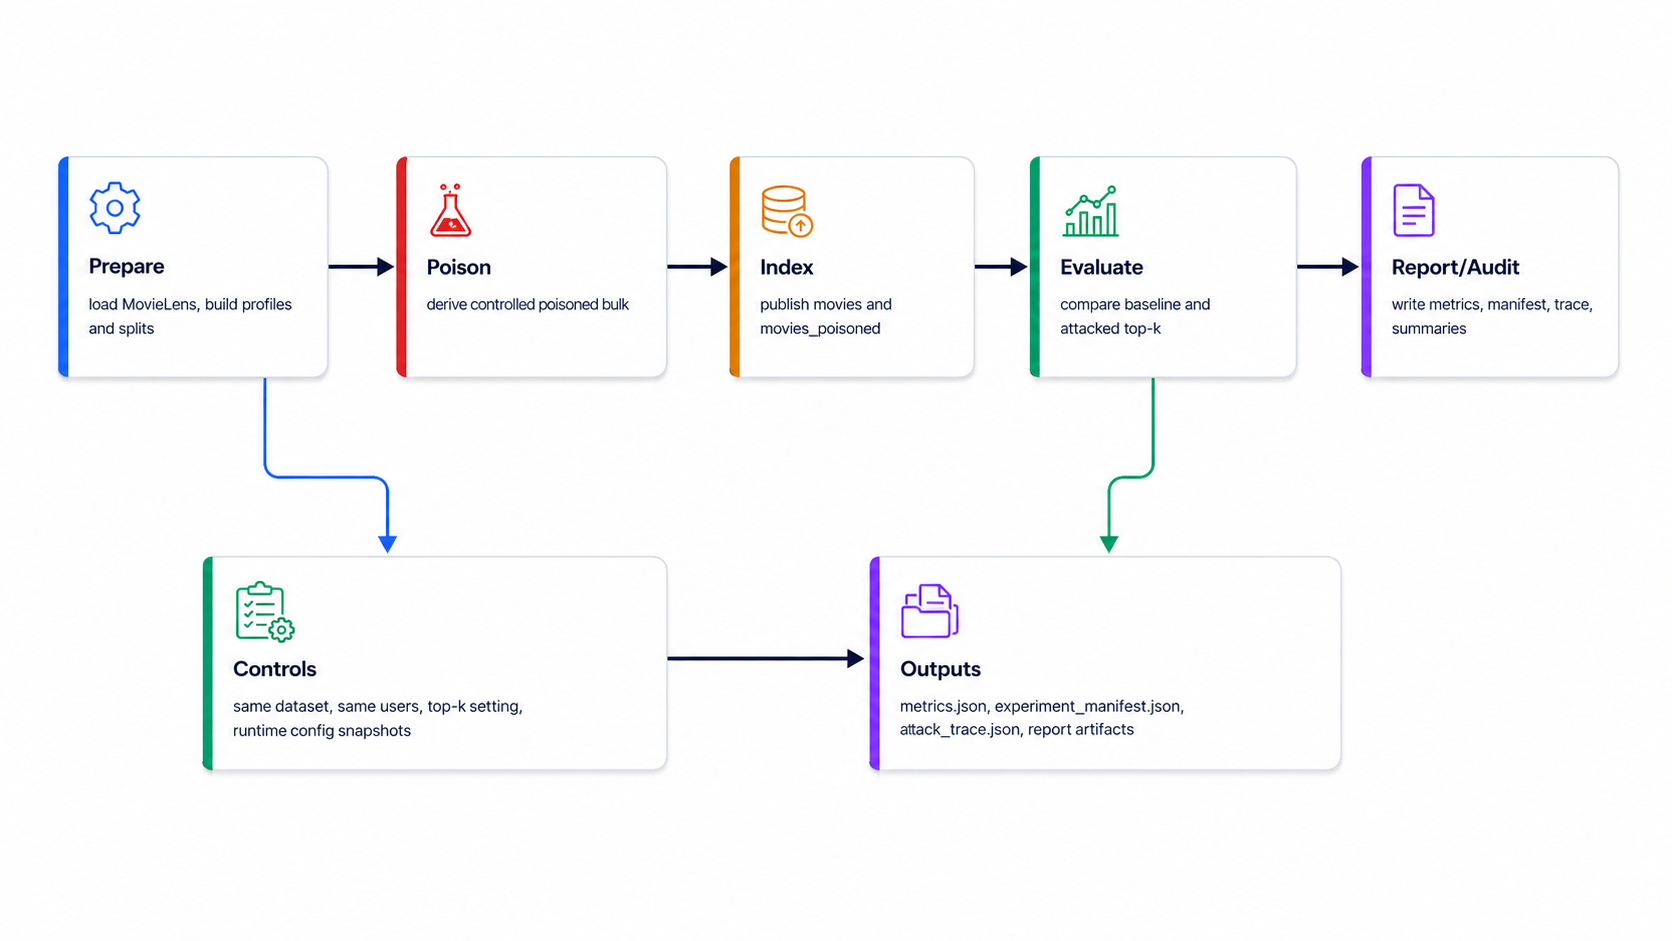
\includegraphics[width=0.92\textwidth]{figures/experiment_lifecycle.png}
  \caption{Experiment lifecycle used to prepare data, build the poisoned corpus, evaluate paired recommendations, and write audit artifacts \cite{ragpoisonlab_repo}.}
  \label{fig:experiment-lifecycle}
\end{figure}

As shown in Figure~\ref{fig:experiment-lifecycle}, the workflow consits of 6 stages six stages. The first stage prepares data where we loaded, normalized, split into training and test portions the MovieLens dataset, then index it through user profile vectors as bulks in Elasticsearch. The second stage builds the poisoned corpus from the attack configuration and applies the attack family on the baseline dataand then index it the poisoned artifact bulk which Then leads to third stage and final indexing steps that lands the clean and poisoned vectors into \texttt{movies} and \texttt{movies\_poisoned} \cite{ragpoisonlab_repo,harper2015movielens,elastic_docs_es}.
The fourth stages is the reccomedation step for both indices on each user, by making a request to Elasticsearch for the top-$k$ values which allows the fifth stage to compute the metrics and write the artifacts that came from the run. the sixth and final stahe generates the necessary inteligeable reports and audit files. all can be executed through the CLI, UI or SDK and does not require commands, though they can help if we need some specific data. In our context the artifact are necessary to accept the experiement as a success as it answers with great detail why and how the results were achieved to document it in this thesis \cite{ragpoisonlab_repo}.

There is a distinction between our final evidence and other runs made through ui, as the full matrix assumes that the production code is stable so there becomes no need to analyze the actual top-$k$ results and only worry about the resuting metrics and the attack parameters as it would be impossible to display them for each of the 943 users at once, but those artifacts are still relevant to show proof of that the system actually works in demo per user runs \cite{ragpoisonlab_repo}.

\subsection{Metrics}

As discussed previously we use the following metrics to calculate our top-$k$ : HR, NDCG, MRR, and ASR. HR is only positive when a movie which shouldnt be at top-$k$ appears in the recommendation and zero otherwise. NDCG mesures if the correct items appear on the list while giving more credits to the ones that appear earlier then compares the results to the best possible ranking \cite{wang2013ndcg}. MRR@K mesures how fast the system finds a correct answer on the list and is zero if it doesnt find any. These metrics are the standard used to evaluate and benchmark the quality of a reccomendation system \cite{herlocker2004evaluating,ragpoisonlab_repo}.

ASR doesnt compute in the same way as the other metrics \cite{ragpoisonlab_repo}. Instead of computing what could essentially be called recommendation health, it insted calculates whether the targeted movie arrives in top-$k$ and if no movie is assigned its value is 0. Targeted promotion could have really high ASR but almost unchanged HR or NDCG while untargeted promotion will have a null value for ASR but really strong results on other metrics.

For each evaluated user $u$, the system implements top-$k$ recommendation list, written as $T_k(u)=(t_1,\ldots,t_{\ell_u})$. Before computing the metrics, invalid movie IDs are ignored and duplicate movie IDs are removed, so the final list can contain fewer than $k$ items, meaning $\ell_u \leq k$. The set $R_u$ represents the user's relevant picked movies, which are used as the ground truth for evaluation and When the attack has a specific target, $c$ represents the configured target movie identifier. THe metrics are calulated using the following formulas \cite{ragpoisonlab_repo,herlocker2004evaluating,wang2013ndcg}:

\[
\mathrm{HR@}k(u)=
\left\{
\begin{array}{ll}
1, & k>0,\ R_u\neq\emptyset,\ \exists i\leq \ell_u : t_i\in R_u,\\
0, & \mathrm{otherwise,}
\end{array}
\right.
\]
\[
\mathrm{NDCG@}k(u)=
\left\{
\begin{array}{ll}
\frac{\sum_{i=1}^{\ell_u}\frac{\mathbf{1}[t_i\in R_u]}{\log_2(i+1)}}{\sum_{i=1}^{\min(|R_u|,k)}\frac{1}{\log_2(i+1)}}, & k>0,\ R_u\neq\emptyset,\\
0, & \mathrm{otherwise,}
\end{array}
\right.
\]
\[
r_u=\min\{i\mid 1\leq i\leq \ell_u,\ t_i\in R_u\},
\qquad
\mathrm{MRR@}k(u)=
\left\{
\begin{array}{ll}
\frac{1}{r_u}, & r_u\ \mathrm{exists},\\
0, & \mathrm{otherwise,}
\end{array}
\right.
\]
\[
\mathrm{ASR@}k(u)=
\left\{
\begin{array}{ll}
1, & k>0,\ c\neq\emptyset,\ c\in T_k(u),\\
0, & \mathrm{otherwise.}
\end{array}
\right.
\]
The run-level value written to the experiment artifacts is the arithmetic mean over the $N$ evaluated users \cite{ragpoisonlab_repo}:
\[
\overline{m@k}=\frac{1}{N}\sum_{u=1}^{N} m@k(u).
\]

\begin{table}[H]
\centering
\small
\begin{tabular}{p{0.24\textwidth}p{0.32\textwidth}p{0.32\textwidth}}
\toprule
Attack family & Primary metric role & Methodological interpretation \\
\midrule
Targeted promotion & ASR plus HR/NDCG/MRR context & ASR indicates target membership in final top-$k$; quality metrics show collateral recommendation effects. \\
Prompt-injection insertion & ASR when target context exists; trace diagnostics & ASR and traces show whether injected/targeted content reaches retrieval and ranking outputs. \\
Untargeted degradation & HR, NDCG, and MRR & Quality metrics show whether poisoning reduces held-out relevance or pushes relevant items lower. \\
\bottomrule
\end{tabular}
\caption{Attack-family metric applicability for the methodology \cite{ragpoisonlab_repo}.}
\label{tab:attack-metric-applicability}
\end{table}

All final results of the full matrix use $k=10$, so the thesis will mostly discuss HR@10, NDCG@10, MRR@10, and ASR@10. RAGPoison allows for configurable $k$ but to simplify the process while getting the most complete results, $k=10$ is a good compromise \cite{ragpoisonlab_repo}.

\subsection{Controls and Reproducibility}

The main source of control is that all runs are made on the same starter data and top-$k$ values and that all steps are recorded. Retrieval and ranking have modular parammeters from retrieval method and its three modes (lexical, dense or hybrid) to ranking modes (deterministic or LLM based). All behavior can be audited and allows deep knowledge of every-step knowing what happened and how to reproduce it \cite{ragpoisonlab_repo}. 

Reproducibility is also supported by clear rules in the code and workflow. The data is split using each user’s timestamp order and the retrieval index names stay fixed. The metrics code uses explicit top-$k$ functions which the report generator reads and then save to the run folders instead of recalculating results from the current live system state. These rules make it easier to rerun parts of the experiment  while being sure that the ouputed result will still match the rest. If the local setup, model provider, or indexed corpus changes, the saved runtime snapshots help explain why the new results may be different \cite{ragpoisonlab_repo}.
